\documentclass{tufte-handout}

\title{Lecture 2: Propositional Probability\thanks{CS7470 Fall 2023: Foundations of Probabilistic Programming.}}

\author[]{Steven Holtzen\\s.holtzen@northeastern.edu}

%\date{28 March 2010} % without \date command, current date is supplied

%\geometry{showframe} % display margins for debugging page layout
\setcounter{secnumdepth}{1}

\usepackage{graphicx} % allow embedded images
  \setkeys{Gin}{width=\linewidth,totalheight=\textheight,keepaspectratio}
  \graphicspath{{graphics/}} % set of paths to search for images
\usepackage{amsmath,amssymb,amsthm}  % extended mathematics
\usepackage{booktabs} % book-quality tables
\usepackage{units}    % non-stacked fractions and better unit spacing
\usepackage{multicol} % multiple column layout facilities
\usepackage{lipsum}   % filler text
\usepackage{fancyvrb} % extended verbatim environments
  \fvset{fontsize=\normalsize}% default font size for fancy-verbatim environments
\usepackage{listings}
\usepackage{tikz}
\usepackage{mathpartir}
\usepackage{subcaption}
\usepackage{mdframed}
\usepackage{epigraph}
\usepackage{enumitem}
\usepackage{stmaryrd}

\usetikzlibrary{shapes.geometric}


\usepackage[ruled,linesnumbered]{algorithm2e}
\SetKwComment{Comment}{/* }{ */}
\newcommand{\indep}{\perp \!\!\! \perp}

\tikzset{
  treenode/.style = {shape=rectangle, rounded corners,
                     draw, align=center,
                     },
  root/.style     = {treenode, font=\Large, bottom color=red!30},
  env/.style      = {treenode, font=\ttfamily\normalsize},
  dummy/.style    = {circle,draw}
}

% tikz
\usetikzlibrary{patterns,calc,backgrounds}


% TIKZ
\tikzstyle{nnf}=[
  >=stealth,font=\small,auto,scale=0.7,every node/.style={scale=0.7}
]
\tikzstyle{extnode}=[
  draw,circle,inner sep=2pt,fill=white
]

\tikzstyle{leafnode}=[
  draw,fill=gray!20,inner sep=3.5pt
]
\tikzstyle{constnode}=[
  draw,fill=white,inner sep=3.5pt
]
\tikzstyle{label}=[
  fill=white,inner sep=2.5pt
]

\tikzstyle{acarrow}=[
    decoration={markings,mark=at position 1 with {\arrow[scale=0.6]{>}}},
    postaction={decorate},
    shorten >=0.4pt,
    >=latex,
    line width=0.1
]

\tikzstyle{bnarrow}=[
    decoration={markings,mark=at position 1 with {\arrow[scale=1.5]{>}}},
    postaction={decorate},
    shorten >=0.7pt,
    >=latex,
    line width=0.3
]
\tikzstyle{bayesnet}=[
  >=latex, thick, auto
]
\tikzstyle{bnnode}=[
  draw,ellipse,minimum size=7mm,inner sep=1pt,font=\small
]
\tikzstyle{cpt}=[
  font=\footnotesize
]

\tikzstyle{graph}=[
  >=stealth,font=\small,auto,scale=1,every node/.style={scale=1}
]
\tikzstyle{node}=[
  draw,circle,inner sep=3pt,fill=white
]

% BDDs

\tikzstyle{bdd}=[
  >=latex, thick, >=stealth, font=\small,auto,scale=0.9,every node/.style={scale=0.9}
]
\tikzstyle{bddnode}=[
  draw,circle,inner sep=0pt,fill=white,minimum size=5.5mm
]

\tikzstyle{bddtriangle}=[
  draw, regular polygon, regular polygon sides = 3,inner sep=1pt,fill=white,minimum size=5.5mm
]

\tikzstyle{highedge}=[
    line width=0.9
]
\tikzstyle{lowedge}=[
    line width=0.9,dotted
]
\tikzstyle{bddterminal}=[
  draw,fill=gray!20,inner sep=2.5pt, font=\small
]

\lstdefinestyle{compact}{
  \ttfamily\tiny
}


\usetikzlibrary{positioning}

\newtheorem{theorem}{Theorem}
\newtheorem{definition}{Definition}
\newtheorem{conjecture}{Conjecture}
\newtheorem{lemma}{Lemma}
\newtheorem{exercise}{Exercise}
\newtheorem{remark}{Remark}


\usepackage{xcolor}

\definecolor{codegreen}{rgb}{0,0.6,0}
\definecolor{codegray}{rgb}{0.5,0.5,0.5}
\definecolor{codepurple}{rgb}{0.58,0,0.82}
\definecolor{backcolour}{rgb}{0.95,0.95,0.92}

\lstdefinestyle{mystyle}{
    backgroundcolor=\color{backcolour},   
    commentstyle=\color{codegreen},
    keywordstyle=\color{magenta},
    numberstyle=\tiny\color{codegray},
    stringstyle=\color{codepurple},
    basicstyle=\ttfamily\footnotesize,
    breakatwhitespace=false,         
    breaklines=true,                 
    captionpos=b,                    
    keepspaces=true,                 
    numbers=left,                    
    numbersep=5pt,                  
    showspaces=false,                
    showstringspaces=false,
    showtabs=false,                  
    tabsize=2
}

\lstset{style=mystyle}

\newcommand{\defn}[1]{\textbf{#1}}
\newcommand{\dbracket}[1]{\left \llbracket {#1} \right \rrbracket}
\newcommand{\dist}[1]{\mathtt{Dist}(#1)}
\newcommand{\true}[0]{\texttt{true}}
\newcommand{\te}[0]{\texttt{e}}
\newcommand{\false}[0]{\texttt{false}}
\newcommand{\real}[0]{\mathbb{R}}
\newcommand{\rational}[0]{\mathbb{Q}}
\newcommand{\lebesgue}[0]{\mathbb{L}}
\newcommand{\eval}[0]{\mathrm{ev}}
\newcommand{\disc}[0]{\textsc{Disc}}
\newcommand{\borel}[0]{\mathcal{B}}
\newcommand{\ent}[0]{\mathbb{S}}
\newcommand{\prog}[0]{\texttt{p}}
\newcommand{\bool}[0]{\mathbb{B}}
\newcommand{\cont}[0]{\textsc{Cont}}
\newcommand{\prop}[0]{\textsc{Prop}}
\newcommand{\bdd}[0]{\textsc{Bdd}}
\newcommand{\robdd}[0]{\textsc{Robdd}}
\newcommand{\compiles}[0]{\rightsquigarrow}

\newcommand{\bddtriangle}[1]{
    \begin{tikzpicture}
    \node [bddtriangle] {#1};
    \end{tikzpicture}}
\newcommand{\bddtrue}[0]{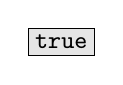
\begin{tikzpicture}
      \node [bddterminal] {$\true$};
    \end{tikzpicture}}
\newcommand{\bddfalse}[0]{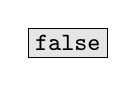
\begin{tikzpicture}
      \node [bddterminal] {$\false$};
    \end{tikzpicture}}


% Standardize command font styles and environments
\newcommand{\doccmd}[1]{\texttt{\textbackslash#1}}% command name -- adds backslash automatically
\newcommand{\docopt}[1]{\ensuremath{\langle}\textrm{\textit{#1}}\ensuremath{\rangle}}% optional command argument
\newcommand{\docarg}[1]{\textrm{\textit{#1}}}% (required) command argument
\newcommand{\docenv}[1]{\textsf{#1}}% environment name
\newcommand{\docpkg}[1]{\texttt{#1}}% package name
\newcommand{\doccls}[1]{\texttt{#1}}% document class name
\newcommand{\docclsopt}[1]{\texttt{#1}}% document class option name
\newenvironment{docspec}{\begin{quote}\noindent}{\end{quote}}% command specification environment



\begin{document}
\maketitle% this prints the handout title, author, and date
\marginnote{``Programming languages are languages, a means of expressing
computations in a form comprehensible to both people and machines.'' \citet{harper2016practical}}



Today we will see an example of our first ``probabilistic programming
language''. I put that in quotes because it is not going to look like a typical
programming language like C or Java. We will build our way up to programming
languages that look more familiar to you, but today we will encounter a ``baby''
PPL that is nonetheless surprisingly useful. That baby PPL will be based on
\emph{propositional logic}. Along the way, we will see the basics of
(discrete) probability that we will need for the first part of the course.

\section{Probability}
\marginnote{``Whereas truth values in logic characterize the formulas under
 discussion, uncertainty characterizes \emph{invisible}
 facts.''
 \citet{pearl1988probabilistic}
}
\marginnote{The formal notion of probability 
used here was introduced by Kolmogorov; see \citet{kolmogorov2018foundations}. 
There have been many introductions and interesting discussions of formal 
notions of probability over the years; see \citet{jaynes2003probability} for an 
interesting discussion. I also like the discussion in \citet[Chapter 8]{graham1989concrete}}
We begin with some formal definitions from \emph{probability}, which will give us a formal basis 
for describing relative degrees of certainty we give to facts about the world:
\begin{definition}
    Let $\Omega$ be a set called the \defn{sample space}; assume that $|\Omega|$ is at most 
    countably-infinite; we will deal with larger classes of sample spaces later on.
    A function $\Pr : \Omega \rightarrow [0,1]$ is called a \defn{probability measure on $\Omega$} 
    if it satisfies that $\sum_{\omega \in \Omega} \Pr(\omega) = 1$.
    The pair ($\Omega, \Pr)$ is called a \defn{discrete probability space}.
\end{definition}

For example, a sample space could be the set of all pairs of six-sided dice rolls:
\begin{align*}
    \Omega_{dice} = \{ (1~1), (1~2), (1~3), \cdots, (6~6)\}
\end{align*}
Then, we would assign a \emph{uniform probability distribution} over all dice
rolls:
\begin{align*}
    \text{For all } \omega \in \Omega_{dice}, \Pr_{dice}(\omega) = 1/36.
\end{align*}
Then, we have a probability space $(\Omega_{dice}, \Pr_{dice})$.
Or, continuing with our propositional example,
Table~\ref{tbl:simple} gives an example of a probability table that describes a
probability distribution over the sample space of instances for a 2-variable
propositional sentence involving variables $x$ and $y$.

\begin{table}
    \centering
 \begin{tabular}{c||c}
    \toprule
    $\omega$ & $\Pr(\omega)$ \\
    \midrule 
    $(\true, \true)$ & 0.1 \\ 
    $(\true, \false)$ & 0.2 \\ 
    $(\false, \true)$ & 0.3 \\ 
    $(\false, \false)$ & 0.4 \\ 
    \bottomrule
\end{tabular}
\caption{A simple probability table.}
\label{tbl:simple}
\end{table}

\begin{marginfigure}
    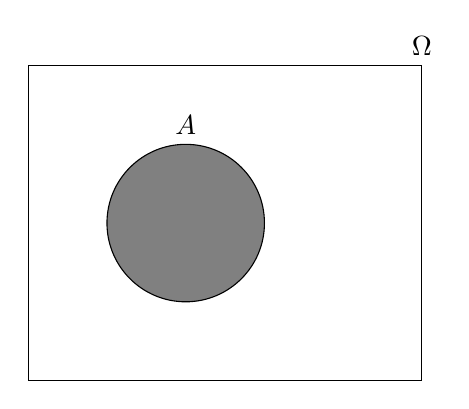
\begin{tikzpicture}
        \draw[fill=gray] (0,0) circle (1) (0,1)  node [text=black,above] {$A$};
            %   (1,0) circle (1) (1,1)  node [text=black,above] {$B$}
        \draw (-2,-2) rectangle (3,2) node [text=black,above] {$\Omega$};
        \end{tikzpicture}
        \caption{An event is a subset of the sample space $\Omega$. Here, the event $A$ 
        is visualized using a Venn-diagram as a subset of the sample space $\Omega$.}
\end{marginfigure}

There is a substantial amount of standard notation for working with probability spaces, 
which we briefly review here; a nice summary resource is \citet[Chapter 3]{darwiche2009modeling}.
An \defn{event} is a subset of the sample space $E \subseteq \Omega$. We define
the probability of an event to be the sum total of all the elements of $\Omega$ that 
are contained in the event:
\begin{align}
    \Pr(E) \triangleq \sum_{\omega \in E} \Pr(\omega).
\end{align}
Continuing with our above example, $\Pr(\{(d_1, d_2) \mid d_1 = 1\})$ is 1/6.

Typically in probability we work with quantities that are derived from the sample space; 
these are called random variables.
Formally, a \defn{random variable} is a map out of the sample space. For instance, we can
define a random variable $S : \Omega_{dice} \rightarrow \mathbb{N}$ to be to sum two dice rolls
$\pi_1$ to be the first die's value, and $\pi_2$ to be the second,where
$\mathbb{N}$ is the set of natural numbers:
\begin{align}
    S((d_1, d_2)) = d_1 + d_2, \quad \pi_1((d_1, d_2)) = d_1, \quad \pi_2((d_1, d_2)) = d_2.
    \label{eq:rvs}
\end{align}

A random variable induces a probability distribution on its co-domain. For a
random variable $X : \Omega \rightarrow D$ acting on a probability space
$(\Omega, \Pr)$, we can compute the probability of a particular element $d \in
D$ by computing the total probability mass in $\Omega$ that is mapped to $d$,
i.e.:\marginnote{Another way of interpreting this notation is that the event $X = x$
is the set of elements of $\Omega$ such that $X(\omega) = x$.}
\begin{align}
    \Pr(X = x) \triangleq \Pr(X^{-1}(x)) = \sum_{\{\omega \in \Omega \mid X(\omega) = x\}} \Pr(\omega).
\end{align}

Given two random variables $X$ and $Y$ defined on the same sample space
$\Omega$, we quite often want to characterize their joint behavior. The 
\defn{joint probability distribution} of two random variables relates them:
\begin{align}
    \Pr(X=x, Y=y) \triangleq \Pr(X^{-1}(x) \cap Y^{-1}(y)).
\end{align}


For example, returning to the dice situation above, we can compute the 
joint probability for any particular pair of dice rolls:
\begin{align*}
    \Pr(\pi_1 = 1, \pi_2 = 1) = \sum_{\{(d_1, d_2) \in \Omega_{dice} \mid d_1 = 1, d_2 = 1 \}} \Pr((d_1, d_2)) = 1/36.
\end{align*}

Given a joint probability distribution $\Pr(X, Y)$, it is often useful to ``forget'' 
one of the random variables and consider only the distribution over the remaining 
variables. This is called the \defn{marginal probability}, and it is computed by summing 
over all possible values the random variable can take on. Concretely, the
marginal probability of $X$ is given by ``summing out'' $Y$:
\begin{align}
    \Pr(X = x) \triangleq \sum_{y} \Pr(X=x, Y=y)
    \label{eq:marg}
\end{align}

\newthought{One of the most common operations} one performs in probability is
\emph{conditioning}: computing the probability that some event happens
\emph{given an observation} that some other event has occurred. For instance,
one might ask, ``what is the probability of that the sum of a pair of dice rolls
is even given that one of them is 1''? Formally, these questions are instances
of \emph{conditional probability}; notationally, the above question would be 
written as $\Pr( S \text { is even} \mid \pi_1 = 1)$; the bar separates two
events, and is read ``given''.


\begin{marginfigure}
    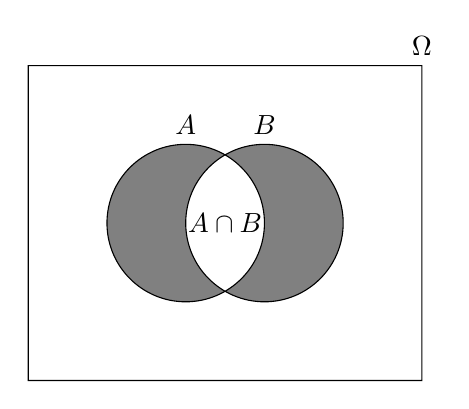
\begin{tikzpicture}[fill=gray]
    % left hand
    \scope
    \clip (-2,-2) rectangle (2,2)
          (1,0) circle (1);
    \fill (0,0) circle (1);
    \endscope
    % right hand
    \scope
    \clip (-2,-2) rectangle (2,2)
          (0,0) circle (1);
    \fill (1,0) circle (1);
    \endscope
    % outline
    \draw (0.5, 0) node {$A \cap B$};
    \draw (0,0) circle (1) (0,1)  node [text=black,above] {$A$}
          (1,0) circle (1) (1,1)  node [text=black,above] {$B$}
          (-2,-2) rectangle (3,2) node [text=black,above] {$\Omega$};
    \end{tikzpicture}
    \caption{It is useful to visualize set intersection when understanding conditioning. 
    By definition, $\Pr(A \mid B) = \Pr(A \cap B)/\Pr(B)$. Intuitively, this corresponds to 
    considering the event at the intersection of these two events, and \emph{re-normalizing}
    that probability based on the viewpoint of the restricted new sample space $B$.
    }
\end{marginfigure}
Given a joint probability distribution $\Pr(X, Y)$, we define the \defn{conditional probability}
of $X$ given $Y$ is:
\begin{align}
    \Pr(X=x \mid Y = y) \triangleq \frac{\Pr(X = x, Y = y)}{\Pr(Y = y)}.
    \label{eq:cond}
\end{align}
There are a number of relationships between these quantities that are commonly used.
One is the law of total probability, which can be derived by
combining equations (\ref{eq:cond}) and (\ref{eq:marg}):
\begin{align}
    \Pr(X=x) = \sum_y \Pr(X = x \mid Y = y)\Pr(y).
\end{align}
It is sometimes the case that conditioning on one random variable has no effect:
for instance, in our dice-roll example, observing the value of the first die
tells you nothing about the value of the second die. Formally, we say two 
random variables $X$ and $Y$ are \defn{independent}, written $X \indep Y$, if 
the following holds:
\begin{align*}
    X \indep Y \text{ if for all }x, y \text{ it holds that } \Pr(X=x \mid Y=y) = \Pr(X = x).
\end{align*}


\begin{exercise}[$\star$]
    See Equation~\ref{eq:rvs}.  What is $\Pr(S = 3 \mid \pi_1 = 1)$?
\end{exercise}

\begin{exercise}[$\star$]
    See Equation~\ref{eq:rvs}. Show that $S \not \indep \pi_1$ and $\pi_1 \indep \pi_2$. 
\end{exercise}

\begin{exercise}[$\star$]
    Let $X$ and $Y$ be random variables defined on the same sample space. Show 
    that, if $X \indep Y$, then $\Pr(X = x, Y = y) = \Pr(X = x) \times \Pr(Y = y)$.
\end{exercise}

\section{Probabilistic models}
One of our main goals in this class is to automate probabilistic reasoning on a
computer.  For this purpose, our discussion so far of probability has been too
abstract: we are told nothing about \emph{how} these various probabilistic
quantities can be computed, or how we can represent probability distributions to
the computer. The means of describing a distribution to a computer is called a
\defn{probabilistic model}; it is a data-structure. The simplest kind of
probabilistic model is a look-up table (or dictionary):
\begin{definition}
    A \defn{probability lookup table} $\mathcal{T}$ is a lookup-table that maps
    elements of the sample space $\omega \in \Omega$ to the probability of that
    element $\Pr(\omega)$. 
    Lookup tables support constant-time lookups.
\end{definition}

For instance, if we are given a discrete sample space with 4 
elements $\Omega = \{1, 2, 3, 4\}$, then we can represent this as 
a dictionary or look-up table:
\begin{align}
    \mathcal{T} = [1 \mapsto 0.1, 2 \mapsto 0.2, 3 \mapsto 0.3, 4 \mapsto 0.4],
\end{align}
The \defn{size} is the amount of memory required to represent the model to the 
computer; it is denoted $|\cdot|$. In the case of a look-up table, the size is 
equal to $|\Omega|$.



\subsection{Querying}
Now that we have a concrete description of a probability distribution, we can
describe algorithms for automatically \emph{querying} for properties about these
representations. Different kinds of probabilistic models will support different 
kinds of queries, and have different complexity-theoretic properties of those queries. cWe have already seen the most basic kind of query: given some 
event $E \subseteq \Omega$, compute the probability of that event $\Pr(E)$. 
This immediately raises the question: how do we represent events? The most basic 
approach is a \defn{set-event}, which supports constant-time membership checks 
(i.e., given some event $\omega \in \Omega$, a set-event $E$ can answer the question 
of whether or not $\omega \in E$ in constant time).
Now, we can give an algorithm for computing the probability of a set-event for 
a particular probability look-up table:

\begin{algorithm}
    \caption{QueryEvent$_1$($\Pr, E)$}\label{alg:eventprob}
    \KwData{A probability look-up table $\Pr$; an set-event $E$}
    \KwResult{The probability of the event $\Pr(E)$}
    $a \leftarrow 0$\;
    \For{each $\omega \in \Omega$}{
        \lIf{$\omega \in E$}{$a \leftarrow a + \Pr(\omega)$}
    }
    \Return{a}
\end{algorithm}

What is the time-complexity of running QueryEvent$_1(\Pr, E)$? Since evaluating
$\Pr(\omega)$ and checking membership $\omega \in E$ are both constant time, the
overall time complexity is $|\Omega|$: the cost of iterating the outer loop from
Lines 2--4.  Is this an acceptable cost? Typically, \emph{no}! The size of the
sample space $\Omega$ is typically prohibitively large: it represents the set of
\emph{all} possibilities. 

This leads us to \emph{the fundamental design challenge of probabilistic modeling}.
We desire a \emph{concise} (i.e., small in representation size, for instance polynomial in $\log |\Omega|$) language for describing 
probability distributions and queries; ideally, this language is usable and interpretable 
by a user. Additionally, we desire we want our queries to be \emph{tractable}: when we 
compute the probability of an event (or perhaps some other kind of query), we want it to 
be as efficient as possible in the representation size. We will see that these two attributes,
tractability and conciseness, are in tension. In the case of lookup-table
distributions and set-events, queries are tractable -- they are typically linear $|\mathcal{T}|$,
but these representations are not concise: they are as large as the sample space.


\section{Propositional logic}

What is a good language for describing probability distributions that is an 
alternative to lookup-table distributions and set-events? Throughout the course 
we will slowly grow our vocabulary for describing these things, but for now we 
begin with a simple language for describing sets of possibilities: \emph{propositional logic}.

Propositional logic is a formal language and has two components: syntax and
semantics. The syntax tells us how to write valid statements in propositional
logic, and the semantics tell us how to interpret those statements. For example, we 
may wish to express the logical statement ``if it rains, then it is wet''. To do 
this, we will introduce two \defn{propositional variables} $r$ and $w$: $r$ is true 
if and only if it is raining, and $w$ is true if and only if it is wet. We can 
relate these two variables by using \defn{propositional connectives}. In the above example, 
we will use the \defn{implication connective} $r \Rightarrow w$, which states that if $r$ is 
true then so is $w$. 

We can summarize these connectives using the following grammar, which tells us how to form 
any \defn{propositional formula} $\varphi, \alpha,$ or $\beta$ in propositional
logic by combining propositional variables
(lower-case letters) with any of the standard propositional connectives (conjunction $land$, disjunction $\lor$, 
unary negation $\neg$, and bi-implication $\Leftrightarrow$):\sidenote{This style of grammar 
is often called Backus-Naur style.}
\begin{align}
    \varphi, \alpha, \beta ::= V \mid \neg \varphi \mid \alpha \land \beta \mid 
    \alpha \lor \beta \mid \alpha \Rightarrow \beta \mid \alpha \Leftrightarrow \beta 
    \mid (\alpha)
\end{align}

Using the above grammar, we can write down some more formulae, like
$(a \land b) \lor (c \land \neg d)$ and $(a \Leftrightarrow b) \land w$.

\subsection{Semantics of propositional logic}
We now know how to write down valid syntactic formulae in propositional logic, but 
we have not yet described what they \emph{mean}: how these formulae relate to the 
original quantities in the real world, and how to unambiguously interpret these various
connectives? Importantly, we want to be able to interpret propositional formulae 
in terms of sets: this will let us connect back to our earlier goals for 
efficiently representing events and distributions.

One way to interpret a formula is by asking if, for a particular state of the
world, is the formula true? To do this, we can fix an \defn{interpretation} $I : V
\rightarrow \{\true, \false\}$, which is a map that maps any variable $v \in V$
to a truth assignment; intuitively, this interpretation will capture some state 
of the world. For example, in our running example, an interpretation that states 
that it is currently raining and not wet would be:\sidenote{As notation, we will sometimes 
abbreviate $r \mapsto \true$ as an unadorned $r$, and $r \mapsto \false$ as
$\overline{r}$. Additionally, we use the notation $\triangleq$ to denote definitional equality.}
\begin{align}
    I_{ex} \triangleq [r \mapsto \true, w \mapsto \false] \triangleq [r, \overline{w}].
    \label{eq:iex}
\end{align}

Now we can interpret propositional formulae for a particular interpretation $I$.
This will be our formal notion of semantics:
\begin{definition}[Semantics of propositional formulae]  
    An instance $I$ is called a \defn{model} for a formula $\varphi$, written $I
    \models \varphi$, if the following inductive description holds:
\begin{align*}
    I &\models a & \text{ iff } I(a) = \true \\
    I &\models \neg \varphi & \text{ iff } I \not{\models} \varphi, \text{ i.e. it is not the case that } I \models \varphi \\
    I &\models \alpha \land \beta & \text{ iff } I \models \alpha \text{ and } I \models \beta \\
    I &\models \alpha \lor \beta & \text{ iff } I \models \alpha \text{ or } I \models \beta \\
    I &\models \alpha \Rightarrow \beta & \text{ iff } I \not{\models} \alpha \text{ or } I \models \beta \\
    I &\models \alpha \Leftrightarrow \beta & \text{ iff } I \models \alpha, I \models \beta \text{ or }  I \not{\models} \alpha, I \not{\models} \beta. \\
\end{align*}
\end{definition}
Now we have a nice formal description of when a formula holds for a 
given interpretation $I$: this is our first example in the course of a 
formal language semantics. Here is an example:
\begin{align*}
    [x, \overline{y}] \models x \lor y, \text{ since } [x, \overline{y}](x) = \true.
\end{align*}

\newthought{Given a logical formula,} it is often useful to determine \emph{the 
set of all models} for that formula. In some sense, this tells us everything 
there is to know about that formula. A common way to do this is via a 
\defn{truth table}, which lists (1) all possible interpretations for a fixed 
set of propositional variables, and (2) whether or not each interpretation 
models a particular formula. For example, we can give the truth table 
for the formula $x \lor \overline{y}$ as:\marginnote{Truth tables as a way of 
reasoning about propositional formulae were introduced by \citet{wittgenstein2013tractatus}.}


\begin{table}
\centering
 \begin{tabular}{c||c}
    \toprule
    $I$ & $ I \models x \lor y?$ \\
    \midrule 
    $x~y$ & $\true$ \\ 
    $x ~ \overline{y}$ & $\true$ \\ 
    $\overline{x}~y $ & $\true$ \\ 
    $\overline{x} ~ \overline{y}$ & $\false$ \\ 
    \bottomrule
\end{tabular}
\caption{A simple truth table.}
\end{table}


\subsection{Propositional probability}
Now we are ready to return to our earlier discussion and ask: \emph{can we use
propositional logic as the basis for an effective probabilistic model}?
The first question is: what is our sample space? It's clear so far that a logical 
choice of sample space is the set of all possibly instances for a fixed set 
of Boolean formulae; this sample space will have size $2^n$, where $n$ is the number 
of propositional variables.
Now, if we want to efficiently evaluate queries over this sample space, we need
need two more components:
\begin{enumerate}
    \item A way to efficiently represent a probability distribution on the sample space;
    \item A way to efficiently represent queries over that sample space.
\end{enumerate}

Let's tackle (1) first. What is an alternative representation of a distribution 
that avoids the space-explosion we saw in the lookup-table representation? We 
will need to be more clever about how we represent probabilities. One useful
choice is to assume that all random variables are \emph{independent from each other}, 
and therefore we can concisely describe a joint distribution over all of them:

\begin{definition}[Fully factorized probabilistic model]
    Let $X_1, X_2, \cdots, X_n$ be jointly independent random variables (i.e.,
    for any pair $X_i, X_j$, it is the case that $X_i \indep X_j$). Then, a
    fully-factorized probabilistic model is a collection of $n$ probability
    lookup tables $\Pr(X_i)$, one for each $i$. The joint probability is computed 
    as $\Pr(X_1, X_2, \cdots, X_n) \triangleq \prod_i^n \Pr(X_i)$.
\end{definition}

Observe that a fully-factorized model only requires $O(\sum_i |X_i|)$ space,
which is significantly smaller than $|\Omega|$.\sidenote{The notation $|X|$
refers to the size of a random variable's co-domain.} This is a big improvement
over plain lookup tables, but it comes at a cost of expressivity: there are some
distributions that cannot be represented in a fully-factorized way.

In the context of propositional logic, there is a natural notion of a
fully-factorized model. Let $\Omega$ be the collection of $n$-element instances.
Then, each propositional variable corresponds to a projection out of that sample
space. Let's call this the \defn{fully factorized propositional distribution}: each 
variable in the theory will be associated with an independent probability of 
being $\true$ or $\false$. For example, we may have to propositional variables $x$ and 
$y$; the fully factorized distribution could be given by two independent lookup tables:
\begin{align}
    [x \mapsto 0.1, \overline{x} \mapsto 0.9], \quad [y \mapsto 0.2, \overline{y} \mapsto 0.8].
    \label{eq:indepdist}
\end{align}
Then, the joint probability $\Pr(x, \overline{y})$ is $0.1 \times 0.8$.

\newthought{Now we return to an earlier question}: how do we efficiently represent 
events in the propositional setting? Events are a subset of the sample space. 
The sample space in propositional probability is the set of all instances. Then, 
we can represent events by \emph{propositional formulae}:
\begin{align}
    \Pr(\varphi) \triangleq \sum_{I \models \varphi} \Pr(\varphi).
\end{align}
For instance, for the fully-factorized 
distribution in Eq.~\ref{eq:indepdist}, we can compute the probability of a 
propositional sentence $x \lor y$ by summing the probability mass over each 
instance that models this formula:
\begin{align}
    \Pr(x \lor y) = \Pr([x, y]) + \Pr([x, \overline{y}]) + \Pr(\overline{x}, y).
\end{align}

This is implemented by the following algorithm:

\begin{algorithm}
    \caption{QueryPropositionalEvent$_1$($\Pr, \varphi)$}
    \KwData{A fully-factorized distribution $\Pr$; a propositional formula $\varphi$}
    \KwResult{The probability of the event $\Pr(\varphi)$}
    $a \leftarrow 0$\;
    \For{each $I \in \Omega$}{
        \lIf{$I \models \varphi$}{$a \leftarrow a + \Pr(\omega)$}
    }
    \Return{a}
    \label{alg:enum}
\end{algorithm}


Unfortunately, QueryPropositionalEvent is \emph{still linear} in the size of
$|\Omega|$ due to the outer loop on Lines 2--4.  In all cases, regardless of the
structure of $\varphi$, we have to consider all all the instances, which will
not scale.

\subsection{Efficiently evaluating queries via search}
How do we avoid scaling in $|\Omega|$ during querying? 
In other words: is it possible to design a scalable automated reasoning strategy 
for our tiny probabilistic programming language that we've made so far, with fully-factorized 
propositional distributions and queries given as propositional formulae?
In the worst case, it
may not be possible to avoid considering all possible instances, but we can 
try to avoid this worst-case explosion by delicately \emph{exploiting the problem 
structure}: in particular, we want to simultaneously exploit the fully-factorized 
structure of the distribution along with the fact that all events are written 
as propositional formulae.

One approach is to \emph{exploit the structure of models of the query
$\varphi$}: sometimes, a query may only have a single model, or perhaps most
instances are models. In these cases, we waste a lot of effort enumerating all
models; it is much more efficient to \emph{search} for the few satisfying instances.

For example, consider the formula $x \lor y$. We can recursively decompose this
formula by branching on assignments to propositional variables:

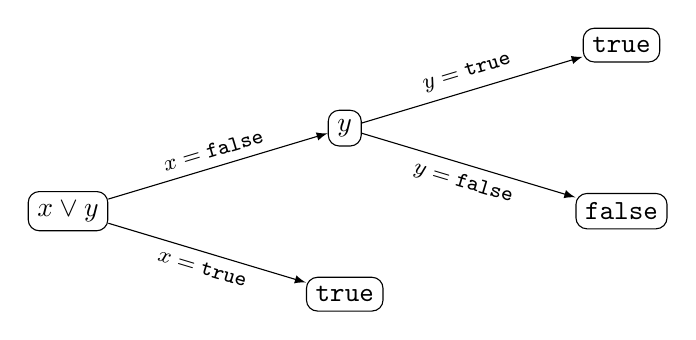
\begin{tikzpicture}
    [
      grow                    = right,
      sibling distance        = 6em,
      level distance          = 10em,
      edge from parent/.style = {draw, -latex},
      every node/.style       = {font=\footnotesize},
      sloped
    ]
    \node [env] {$x \lor y$}
      child { node [env] {$\true$}
        edge from parent node [below] {$x = \true$} }
      child { node [env] {$y$}
        child { node [env] {$\false$}
          edge from parent node [below] {$y = \false$} }
        child { node [env] {$\true$}
                edge from parent node [above, align=center]
                  {$y = \true$}}
                edge from parent node [above] {$x = \false$} };
  \end{tikzpicture}

The root of this binary tree is the original formula $x \lor y$. Each branch 
assigns a propositional variable to a Boolean value. The children are 
the resulting formula evaluated on the \emph{partial instance} given by the 
path up until that point: for instance, if we assign $x = \false$, we are left 
with the formula $\false \lor y = y$. Leaves of the tree denote whether or not a 
particular assignment is a model.\sidenote{% source: https://tex.stackexchange.com/questions/188183/latex-under-construction-in-work-or-work-in-progress-symbols
\scalebox{0.5}[0.5]{
    (under construction)

\begin{tikzpicture}[limb/.style={line cap=round,line width=1.5mm,line join=bevel}]
\draw[line width=2mm,rounded corners,fill=yellow] (-2,0) -- (0,-2) -- (2,0) -- (0,2) -- cycle;
\fill (1.5mm,7mm) circle (1.5mm);
\fill(0,-7.5mm) -- ++(10mm,0mm) -- ++(120:2mm)--++(100:1mm)--++(150:2mm) arc (70:170:2.5mm and 1mm);
\draw[limb] (-7.5mm,-6.5mm)--++(70:4mm)--++(85:4mm) coordinate(a)--++(-45:5mm)--(-2.5mm,-6.5mm);
\fill[rotate around={45:(a)}] ([shift={(-0.5mm,0.55mm)}]a) --++(0mm,-3mm)--++
        (7mm,-0.5mm)coordinate(b)--++(0mm,4mm)coordinate(c)--cycle;
\draw[limb] ([shift={(-0.6mm,-0.4mm)}]b) --++(-120:5mm) ([shift={(-0.5mm,-0.5mm)}]c) --++
        (-3mm,0mm)--++(-100:3mm)coordinate (d);
\draw[ultra thick] (d) -- ++(-45:1.25cm);
\end{tikzpicture}
}}

% this can be described using big-step!
\begin{algorithm}
    \caption{PrEvent($\Pr, \varphi$)}
    \KwData{A fully-factorized distribution $\Pr$; a propositional formula $\varphi$; a decision order $\sigma$.}
    \KwResult{The probability $\Pr(\varphi)$.}
    \lIf{$\varphi = \true$}{\Return 1}
    \lIf{$\varphi = \false$}{\Return 0}
    $v \leftarrow head(\sigma)$\;
    $\sigma' \leftarrow tail(\sigma)$\;
    $ \varphi_v \leftarrow $ fix $v = \true$ in $\varphi$\;
    $ \varphi_{\overline{v}} \leftarrow $ fix $v = \false$ in $\varphi$\;
    \Return{$\Pr(v) \times $PrEvent$(\Pr, \varphi_v) + \Pr(\overline{v}) \times $PrEvent$(\Pr, \varphi_{\overline{v}})$}
    \label{alg:rec}
\end{algorithm}

You should convince yourself that the above algorithm is correct by trying it on a few examples. 
It is a good exercise to prove it correct inductively.
What is the runtime of Algorithm~\ref{alg:rec}? In the worst-case, it is still $|\Omega|$. But, 
sometimes -- depending on the structure of $\varphi$ -- it can do better by terminating the 
recursion earlier in a base-case on Lines 1 and 2, rather than exhaustively exploring all 
instances like Algorithm~\ref{alg:enum}.



% Now, suppose we are given a probability measure $\Pr$ on instances. Now we want
% to ask: \emph{what is the probability that a particular sentence $\varphi$ is
% true for this world?} A subset of $\Omega$ is called an \defn{event}, and the 
% probability of this particular event can be computed as the total probability of
% all models of $\varphi$:
% \begin{align}
%     \Pr(\varphi) \triangleq \sum_{I \models \varphi} \Pr(I).
%     \label{eq:pr2}
% \end{align}
% Note that above we overloaded the notation used for $\Pr$ to now act 
% on events; this is common practice.
% As an example, using the probability measure given in Table~\ref{tbl:simple}, we
% can compute:
% \begin{align}
% \Pr(x \lor y) = \Pr([x, y]) + \Pr([x, \overline{y}]) + \Pr(\overline{x}, y) = 0.6.
% \end{align}

% \subsection{A propositional probabilistic programming language}
% Tables like Table~\ref{tbl:simple} are a very inconvenient way to describe a
% probability distribution. They are exponential in size, making them infeasible 
% to write down for a large set of propositional variables, and they convey no useful 
% structure to the user. In short, tables aren't a very useful probabilistic 
% programming language.

% It is much more convenient and usable 

\begin{exercise}[$\star$]
Give the truth table for $(a \Leftrightarrow b) \land (\neg c).$ 
\end{exercise}
\begin{exercise}[$\star$]
    Give an example of a joint probability distribution that cannot be 
    represented in a fully-factorized way.
\end{exercise}
\begin{exercise}[$\star$]
    Assume the following fully-factorized distribution on propositional variables:
    \begin{align*}
        [x \mapsto 0.1, \overline{x} \mapsto 0.9],\quad [y \mapsto 0.3, \overline{y} \mapsto 0.7].
    \end{align*}
    Use an exhaustive search tree to compute $\Pr(x \Leftrightarrow y)$.
\end{exercise}
\begin{exercise}[$\star\star$]
    Prove Algorithm~\ref{alg:rec} correct.
\end{exercise}



\bibliographystyle{plainnat}
\bibliography{../bib}

\end{document}